%%%%%%%%%%%%%%%%%%%%%%%%%%%%%%%%%%%%%%%%%%%%%%%%%%%
% visualization.tex
%%%%%%%%%%%%%%%%%%%%%%%%%%%%%%%%%%%%%%%%%%%%%%%%%%%
% \subsection{Visualization}\label{sec:viz}

\Gfour{} visualization capabilities \cite{vis:Allison} have been extended to
leverage new user interface technologies, such as Qt \cite{vis:Qt}, and to 
extend many features in response to user needs.  In many cases, visualization 
solutions that previously required extensive user coding are now provided 
through rich built-in functionality. \Gfour{} offers the user many options for
visualization drivers, some of which are always installed, others of which 
require that the user's system include particular external libraries.  
Available visualization drivers include the basic OpenGL-based \cite{vis:OGL}
drivers (OGLX, 
OGLWin32 and OGLXm), three OpenGL drivers which are more interactive (Qt, 
OpenInventor \cite{vis:OI} and OIXE) and the file-based drivers HepRApp 
\cite{vis:HPRP}, RayTracer, DAWN \cite{vis:DAWN}, VRML \cite{vis:VRML},
gMocren \cite{vis:gMoc} and ASCIITree.  Some of these drivers and new features
are detailed below.

\subsubsection{Advances in drivers and viewers}\label{sec:drv}
% Drivers.tex
The workhorses of the \Gfour{} visualization system continues to be its OpenGL
drivers.  Multiple OpenGL drivers are provided because different implementations
are required on different operating systems or for different user memory 
configurations.  For example, one flavor of OpenGL driver offers higher refresh
speed at the cost of using more memory, while another conserves memory at the
cost of speed.  The user experience has been simplified so that it is no longer 
necessary to specify which driver to use (such as /vis/open OGLI or 
/vis/open OGLSWin32).  Instead a single command (/vis/openOGL) may be issued 
from which \Gfour{} will select the most appropriate and capable viewer for the
user's current system.

Other improvements include speed increases through the streamlining of the set
of OpenGL instructions, and the ability to print any OpenGL view to high quality
output by exploiting the GL2PS \cite{vis:GL2PS} OpenGL to PostScript printing 
library.  OpenGL drivers in X11 and Qt modes allow the user to select (``pick'')
objects from the GUI in order to interrogate visualized objects, thus obtaining
track, hit or geometry information.

\Gfour{} now supports wrapping an OpenGL viewer within the versatile, highly
interactive and platform-independent Qt user interface framework.  An example of
this is shown in Figure \ref{fig:vis1}.

\begin{figure}
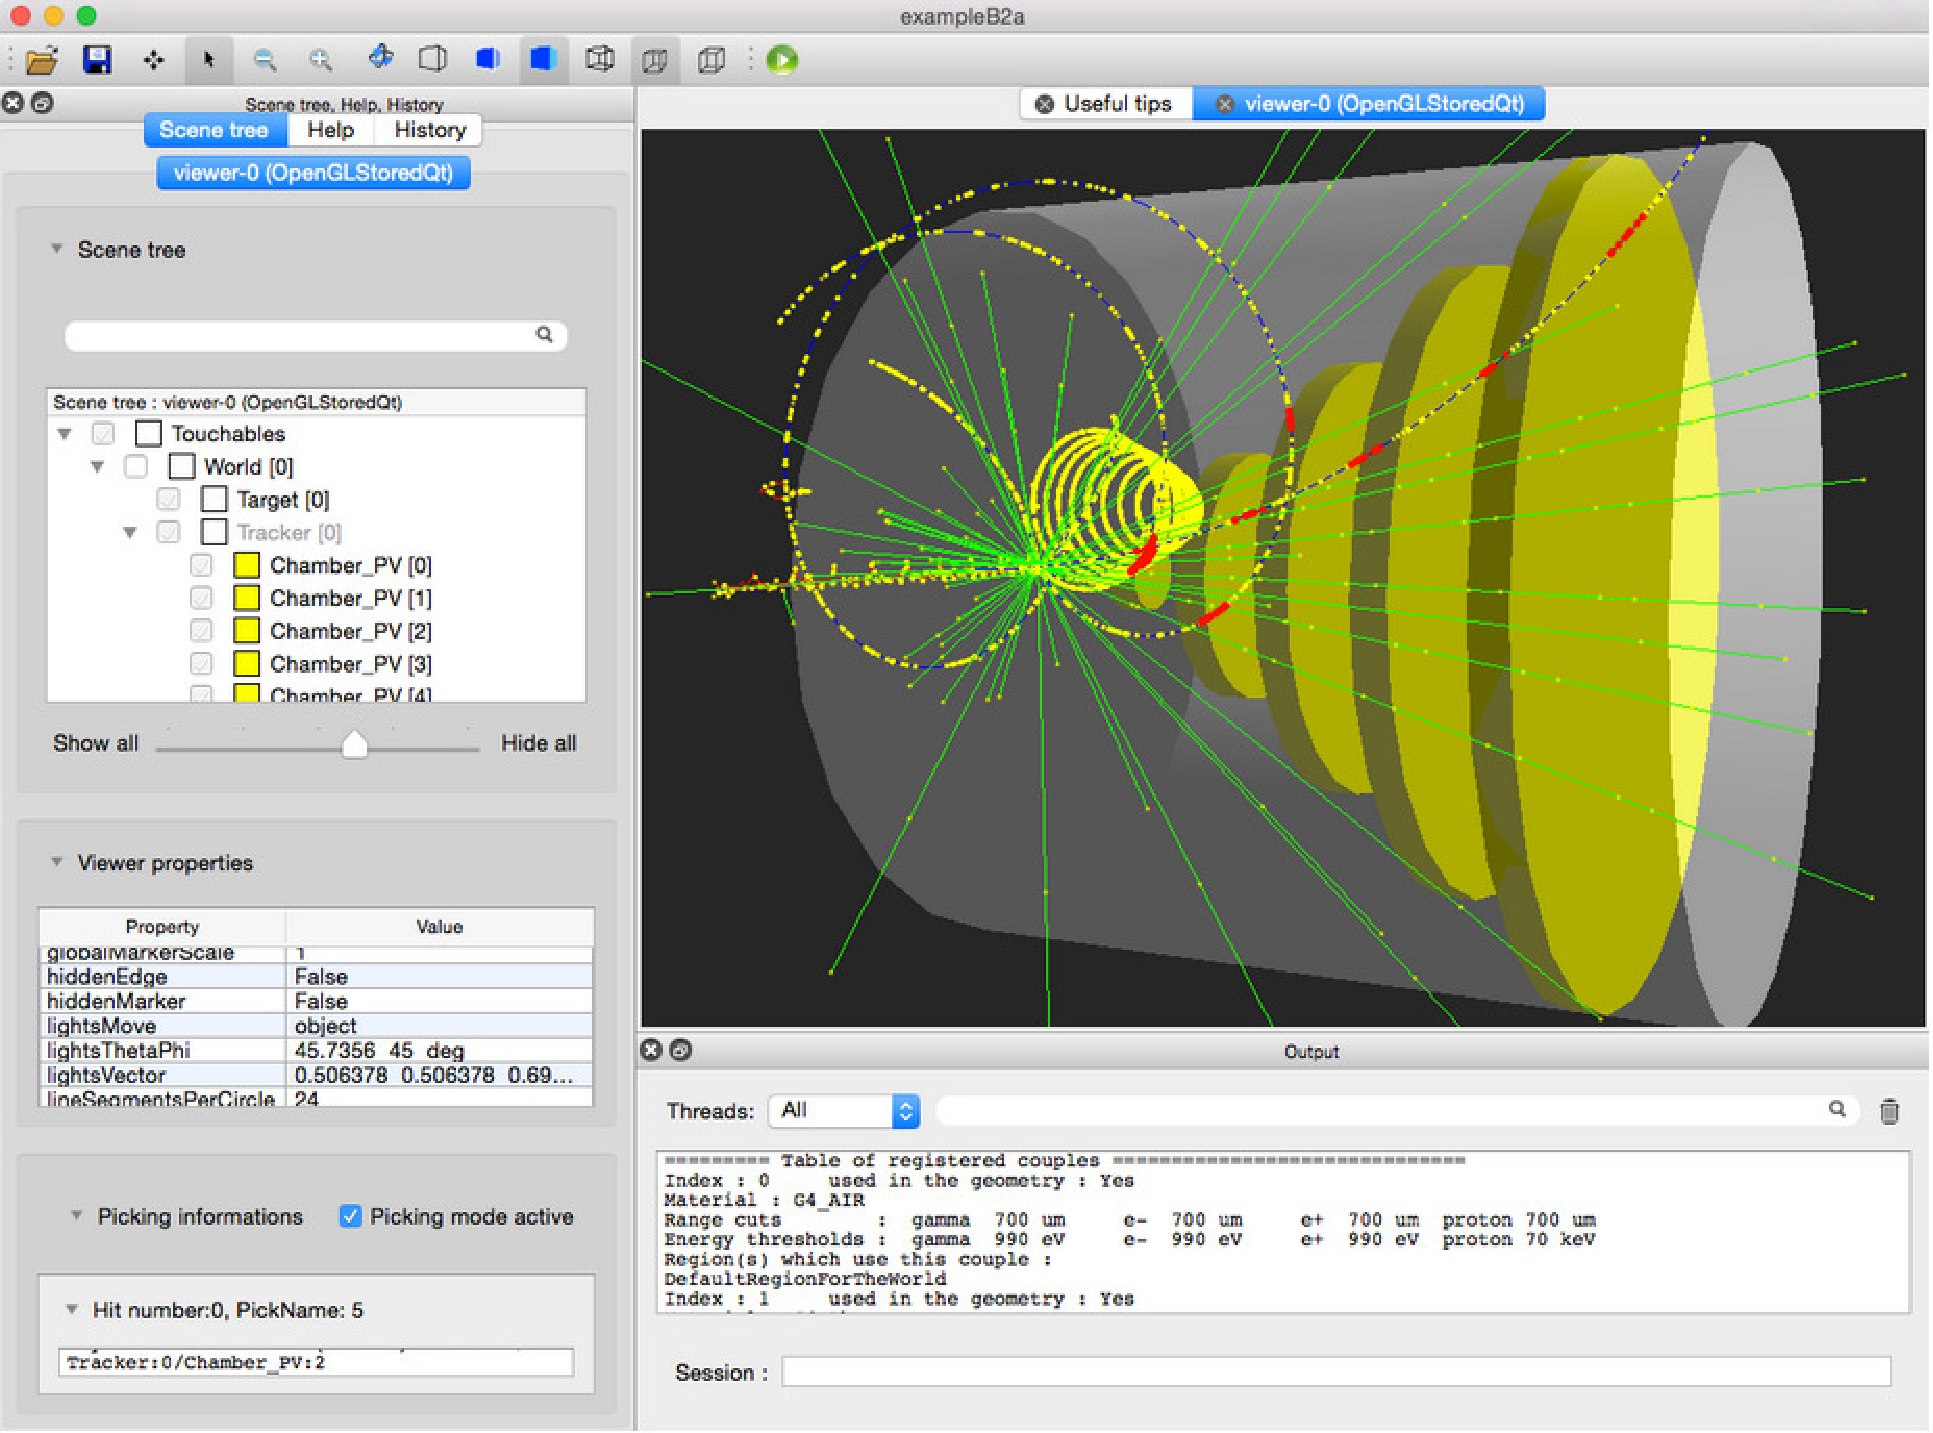
\includegraphics[width=0.47\textwidth]{figures/visfig1.pdf}
  \caption{Screenshot of OpenGL viewer wrapped in Qt.}
  \label{fig:vis1}
\end{figure}
This Qt implementation includes GUI functionality to rotate, zoom and translate
the view, and to pick visualization objects.  A slider lets the user visually
``melt away'' layers of hierarchical geometries.  Movies and EPS output are 
easily generated.  A hierarchical view of the scene's graphical elements allows 
the user to inspect and modify the color and visibility of each element.  
Another hierarchical view provides easy access to the full \Gfour{} help system.

\begin{figure}
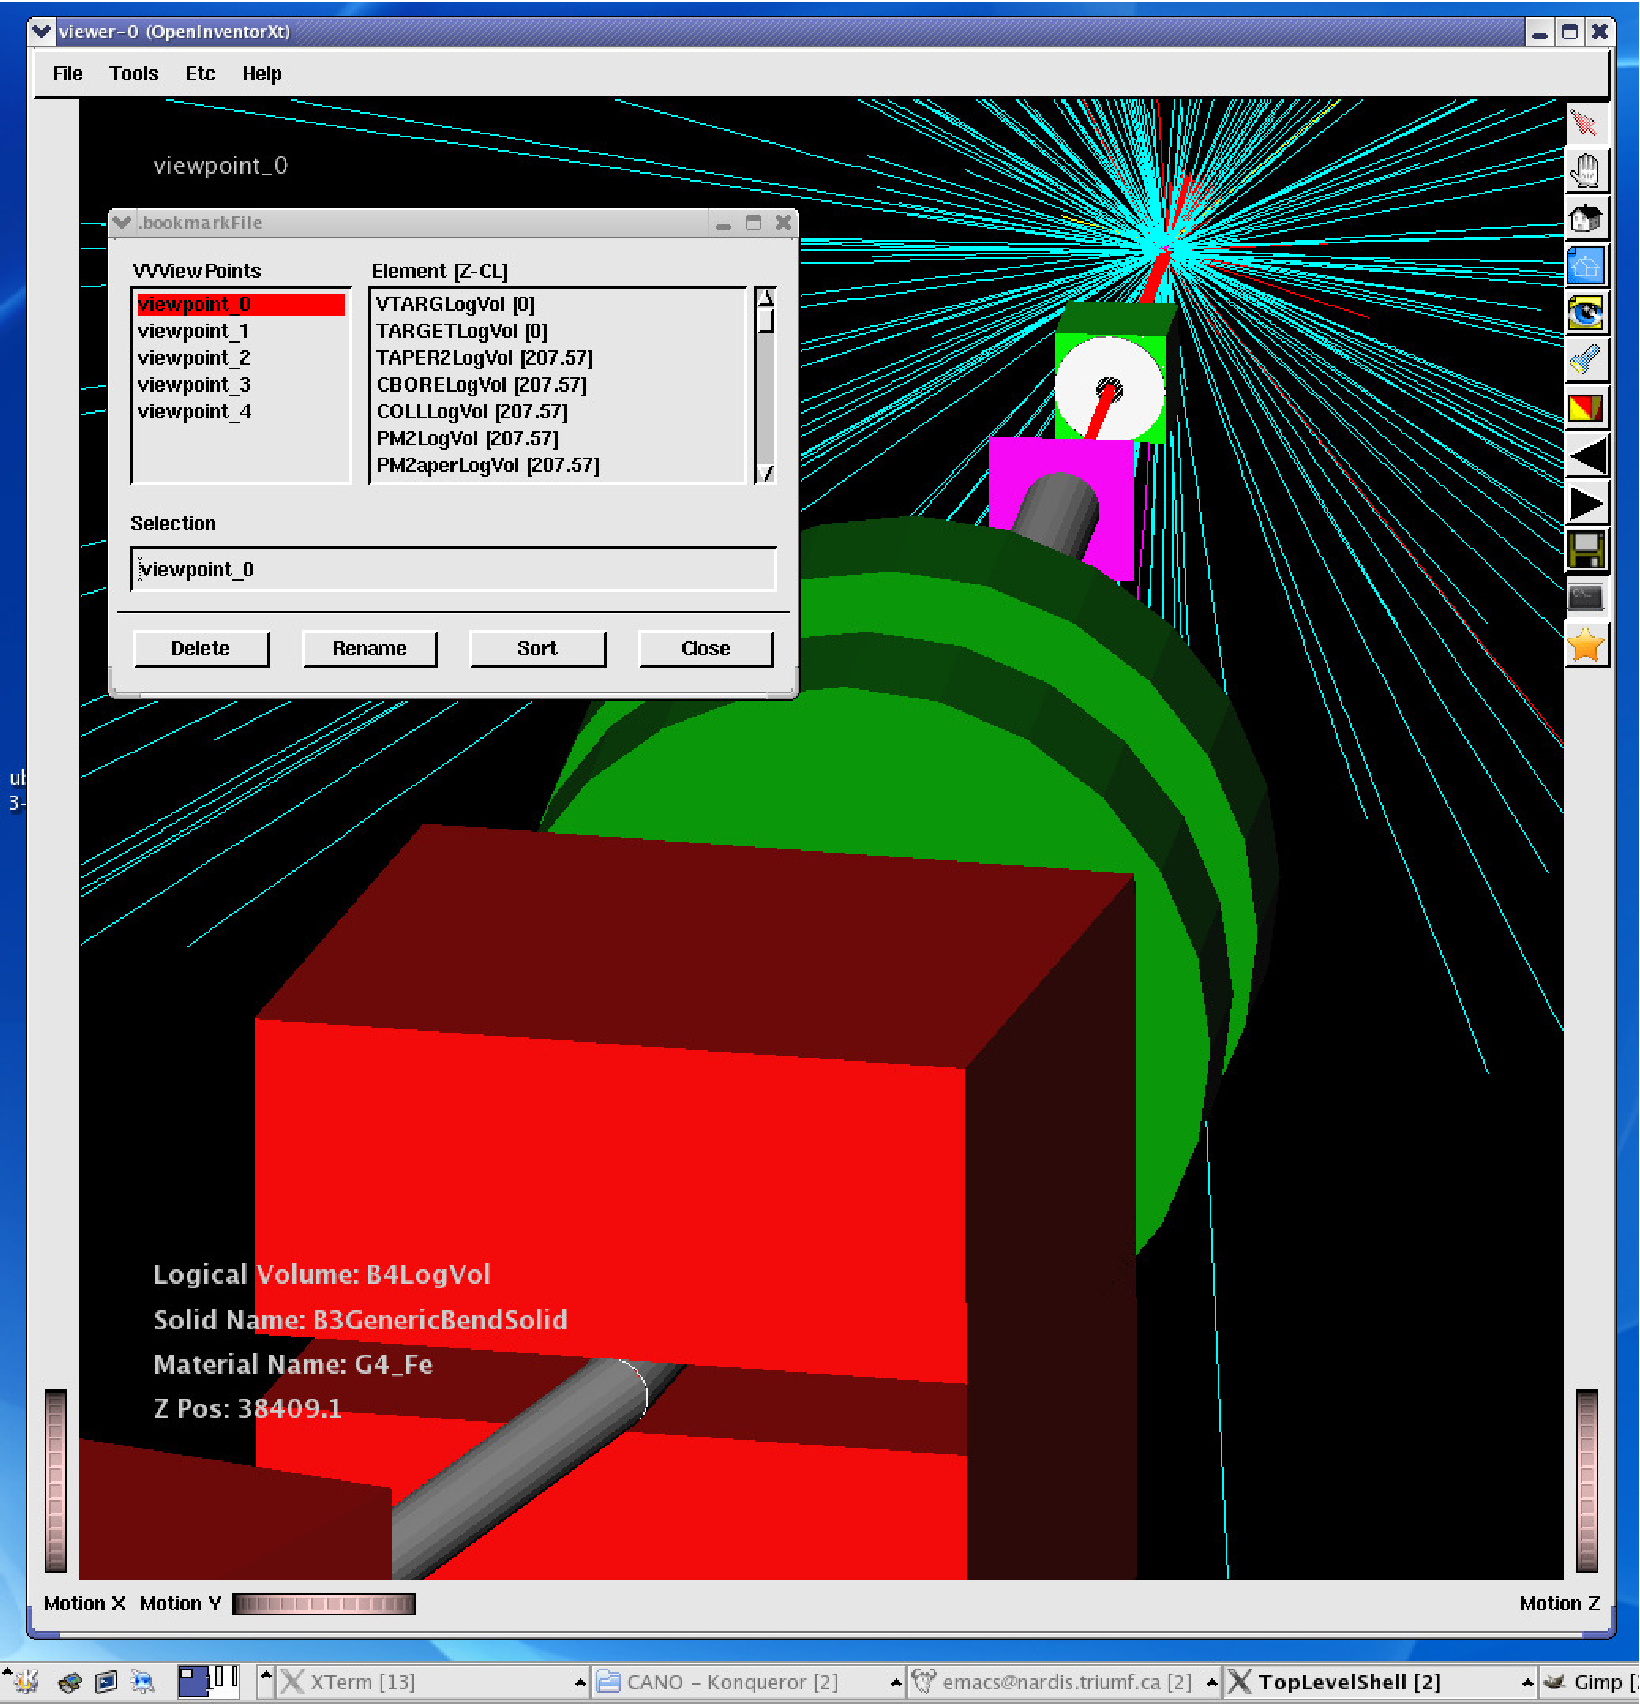
\includegraphics[width=0.47\textwidth]{figures/visfig2.pdf}
  \caption{Screenshot of Open Inventor Extended viewer.}
  \label{fig:vis2}
\end{figure}

New features have also been added to the Open Inventor (OI) driver.  The 
availability of OI greatly improved in 2011 when the Coin3D \cite{vis:coin3d} 
version of these libraries became open-source and freely available.  \Gfour{} 
made extensive use of the Coin3D classes that extend the original SGI OI 
library, creating a distinct new ``extended'' driver OIXE while leaving the 
basic driver OIX unchanged.  Figure \ref{fig:vis2} shows an example of the OIXE
viewer. 

A feature implemented in this area was the ability to save the current view and
return to it at any later time in the current or future runs.  Views are saved 
and accumulated in a bookmarks file specified by the user.  Each view is tagged
with a user-provided or default name, and all views are listed in a scrolling 
auxiliary window.  Clicking on a view name restores the view, or a sequence of 
views can be walked through via the keyboard's arrow keys.  All viewpoint and 
camera parameters are stored in ASCII form allowing editing or external 
generation of bookmarks.

As in other OpenGL viewers, object selection from the GUI is supported on 
trajectories, hits and geometry.  The OI driver provides both normal trajectory 
picking, where all trajectory points are shown, and reduced picking, where only
the first and last points are shown.  The viewer also supports mouse-over 
picking, whereby the element data is displayed directly in the viewer window 
when the mouse pointer is hovered over any object.

The remaining new developments concern moving the camera along a reference
path.  They are motivated by accelerator and beam line geometries, but may be
useful for other large and/or extended structures.  The reference path, defined
in a piecewise linear fashion by an ordered set of points, may be read from a 
file or copied from any particle trajectory.  Once a reference path is 
established, a navigation panel lists all elements in the geometry, ordered by
their distance along the reference path (based on the shortest distance 
\cite{vis:polyline} from the element center to the path).  The panel may then
be used to extract information on the elements or rotate the camera around them.
% moves the camera immediately to a centered view of that 
% element, and the arrow keys can then be used to rotate the camera around the 
% element in precise 90-degree steps around the local axes.  The shifted left and
% right arrow keys provide smooth movement of the camera along the reference path.
% OI capabilities have been used to render these motions smoothly so as not to be
% jarring to the eye.  During camera movement, a continuous readout of the 
% distance along the reference path is given.

A Reference Path Animation mode moves the camera continuously along the path, 
allowing a fly-through giving a particle's-eye view of the geometry.  Keyboard 
controls adjust animation speed and direction and allow adjusting the camera 
angle to obtain fly-overs and fly-unders.



\subsubsection{New feautures in trajectory modeling and filtering}\label{sec:trajectory}

Many options are now provided for how trajectories should be modeled (how colors
or line styles are selected).  These improvements have eliminated the most 
common reason users had to code their own trajectory classes.  In addition to 
the default model, where trajectories were colored by charge, one can now set 
color or other line properties based on particle ID, particle origin volume, or
any other particle attribute that has been loaded into a \texttt{G4AttValue}.
One can also add entirely new, customized trajectory models.  New options make
it easy to control whether trajectories are shown as basic lines, lines plus
step points or step points alone, and one may also modify step point colors.

Additional new features allow trajectories to be filtered, causing only a 
specific subset to be drawn.  These filtering options match the design of the 
trajectory modeling options, so that filtering based on charge, particle ID, 
particle origin volume, or some custom aspect, is possible.  Filters may be
daisy-chained so that one may show, for example, only the neutrons originating
from a particular collimator.

Completing the set of additions to trajectory drawing is the ability to select
smooth and rich trajectories.  By default, trajectories are represented as a set
of line segments connecting particle steps.  Because \Gfour{}'s efficient 
stepping algorithm may require very few steps in some magnetic fields, the 
default trajectory drawn through a solenoidal field may appear very jagged.  The
optional Smooth Trajectory Drawing causes additional points to be generated
along the particle trajectory so that the visualization is smoother.  Rich 
trajectories concern the amount of additional information with which 
trajectories and step points are annotated.  By default, trajectories have only 
basic information attached and step points have only position information; thus 
when one picks on these objects in the various pick-enabled viewing systems 
(HepRApp, Qt, OI or OpenGL with X11), one discovers only a few pieces of 
information about the trajectory and no details about the trajectory points.  
The Rich trajectory option enriches this annotation, providing picked 
trajectories containing many more pieces of information, such as the entire 
history of geometry volumes traversed.  It also adds a wealth of information to
step points, such as the type of process that created the step.



\subsubsection{Additional new features}\label{sec:morefeatures}

% NewFeatures.tex
Time Slicing was added to allow one to produce movies that show the time
development of an event.  With time slicing enabled, the OpenGL line segments
that represent a particle trajectory are annotated with time information.  Users
can then select an OpenGL view that corresponds to a given time, and a sequence
of such views produces the frames of a time development movie.  Users can 
produce these movies in any OpenGL viewer by the appropriate use of \Gfour{}
command macros.  The Qt driver provides a simplified way for users to make such
movies.

\Gfour{} visualization now has the ability to retain the pointers to 
previously-viewed events, so that after visualizing a set of events, one can go
back to the beginning of the set and review the events.  When coupled with 
customized user code that specifies which events should be kept, one can 
potentially run a very large set of events and then afterwards choose to 
visualize only those events that satisfied some personal set of trigger 
conditions.

The following features have also been added:
\begin{itemize}
\item parallel worlds, including layered mass worlds, may now be viewed
      individually or superimposed on the main geometry world;

\item magnetic fields may be displayed as a set of arrows indicating local
      field direction, with arrow lengths proportional to field strength;

\item decorations are now supported which allow the user to easily annotate
      graphical views with text (placed either in 3D coordinates or 
      in the 2D coordinates of the graphics window), run and event number,
      arrows, axes, rulers, date stamps and logos;

\item users may adjust the visibility or appearance of geometry by using the 
      /vis/geometry commands which globally modify the appearance of some set of
      geometry objects, while the /vis/touchable commands allow control of these
      objects individually.
\end{itemize}



\subsubsection{Approach to MT}\label{sec:approachMT}

The final set of changes concern \Gfour{}'s migration to multithreaded (MT) 
operation.  The overall design of visualization remains little-changed for 
those users running in sequential mode, but significant changes were required 
to enable visualization from MT mode.

Currently in MT mode, events are only drawn at end of run, that is, once all
threads have completed their work.  This limitation is scheduled to be removed
in release 10.2 by moving part of visualization to its own thread, such that 
each event is available for drawing as soon as that event is complete.

In MT mode, visualization will properly handle any commands that request drawing
of high level graphical objects (geometry volumes, trajectories and decorations
such as axes).  However, user-supplied code that directly asks the visualization 
system to draw low level graphical primitives (polygons or polylines) is not 
supported.  This limitation will not likely affect many \Gfour{} users, as 
recent improvements to geometry, trajectory and decoration handling have made 
such user-supplied code largely unnecessary.  Because significant work will be 
required to remove this limitation, support will come only if there is strong 
demand for these features in MT mode.

The RayTracer driver has itself been been multithreaded to take maximum 
advantage of MT.



